\chapter{KẾT QUẢ VÀ BÀN LUẬN}
\label{ch:ket_qua}

\section{Kết quả tổng quan}

\subsection{Hai giai đoạn thực nghiệm}
\label{sec:quy_uoc_do}

Đề tài được tiến hành qua \textbf{hai giai đoạn} có mục tiêu khác nhau, và điều này quyết định cách
đọc các bảng số liệu phía sau.

\textbf{Giai đoạn một} tập trung vào phân tích dữ liệu và thiết lập mốc so sánh. Câu hỏi đặt ra là
hai họ kiến trúc lớn --- tích chập một giai đoạn và transformer dự đoán theo tập hợp --- khác nhau
ra sao trên bộ dữ liệu này. Đây là nội dung của nhóm E0, với YOLOv8n đối đầu DETR-ResNet50. Kết quả
được ghi ra tệp chỉ số bởi mô-đun đánh giá, lưu kèm đường dẫn trọng số, tên tập đánh giá và thiết bị
đo, nên truy vết được đầy đủ.

\textbf{Giai đoạn hai} chuyển trọng tâm sang bài toán triển khai. Sau khi giai đoạn một đã cho thấy
DETR không hội tụ kịp trong ngân sách hiện có, việc tiếp tục so với DETR không còn giá trị thông
tin; câu hỏi mới trở thành làm sao đưa mô hình tốt nhất xuống phần cứng hạn chế. Đó là lý do các
nhóm E1, E2 và E3 so sánh với những đối tượng khác --- kiến trúc nhẹ, mô hình lượng tử hoá, mô hình
chưng cất --- thay vì với DETR.

Vì hai giai đoạn cách nhau về thời gian và chạy trên hai cấu hình phần cứng khác nhau, \emph{các con
số giữa hai giai đoạn không so sánh trực tiếp được với nhau}. Cấu hình YOLOv8n xuất hiện ở cả hai và
cho hai bộ số: 0,9539 với 113,2 khung hình mỗi giây ở giai đoạn một, so với 0,9633 và 65,3 ở giai
đoạn hai. Báo cáo \emph{không} chọn một con số rồi bỏ con số kia, mà ghi nhận cả hai kèm nhãn giai
đoạn, và mọi phép so sánh chỉ được thực hiện \emph{trong nội bộ từng giai đoạn}.

\subsection{Bảng tổng hợp}

\begin{table}[H]
\centering
\caption{Tổng hợp kết quả bốn nhóm thực nghiệm trên tập kiểm tra}
\label{tab:tongquan}
\footnotesize
\begin{tabular}{clp{3.9cm}rrrc}
\toprule
\textbf{Mã} & \textbf{Cấu hình} & \textbf{Cách làm} & \textbf{mAP@0,5} & \textbf{mAP@0,5:0,95} & \textbf{FPS} & \textbf{GĐ} \\
\midrule
\multicolumn{7}{l}{\textit{Giai đoạn 1 --- mốc so sánh giữa hai họ kiến trúc}} \\
E0 & \textbf{YOLOv8n}      & Mô hình nền, 30 chu kỳ            & \textbf{0,9539} & \textbf{0,8058} & 113,2 & 1 \\
E0 & DETR-ResNet50         & Transformer nền, 10 chu kỳ        & 0,1220 & 0,0988 & 15,7  & 1 \\
\midrule
\multicolumn{7}{l}{\textit{Giai đoạn 2 --- bài toán triển khai, phần cứng khác}} \\
-- & YOLOv8n FP32          & \textit{Mốc tham chiếu giai đoạn 2}  & \textit{0,9633} & \textit{0,8068} & \textit{65,3} & 2 \\
E1 & YOLO11n               & Thế hệ YOLO mới hơn, nhẹ hơn      & 0,9252 & 0,7833 & 59,0 & 2 \\
E1 & SSDLite-MobileNetV3   & CNN di động, 320 điểm ảnh         & 0,7432 & 0,6260 & 57,9 & 2 \\
E1 & D-FINE-Nano           & Transformer thế hệ mới, nhẹ       & 0,7836 & 0,6589 & 25,8 & 2 \\
E2 & PyTorch FP16          & Giữ YOLOv8n, đổi sang FP16        & 0,9633 & 0,8068 & 65,3 & 2 \\
E2 & ONNX INT8             & Lượng tử hoá sau huấn luyện       & 0,9552 & 0,7973 & 5,7  & 2 \\
E2 & OpenVINO INT8         & INT8 qua OpenVINO trên CPU        & 0,9265 & 0,7846 & 13,9 & 2 \\
E3 & YOLO26n đối chứng     & Học trò huấn luyện thường, 50 chu kỳ & 0,9348 & 0,7773 & 69,7 & 2 \\
E3 & YOLO26n chưng cất     & Học từ YOLO26s, hệ số 6,0         & 0,9014 & 0,7450 & 74,8 & 2 \\
\bottomrule
\end{tabular}
\end{table}

\hopnhanmanh{Trong nội bộ giai đoạn 2, không một cấu hình nào trong tám cấu hình khảo sát vượt được
mốc tham chiếu YOLOv8n FP32. Kết quả này đi ngược giả thuyết ban đầu ở cả nhóm E1 lẫn nhóm E3, và
được báo cáo đầy đủ ở Mục~\ref{sec:trai_ky_vong}.}

\section{E0 --- So sánh mô hình nền}

\subsection{Kết quả chi tiết}

\begin{table}[H]
\centering
\caption{So sánh chi tiết YOLOv8n và DETR-ResNet50 trên tập kiểm tra}
\label{tab:e0}
\small
\begin{tabular}{lrr}
\toprule
\textbf{Chỉ số} & \textbf{YOLOv8n} & \textbf{DETR-ResNet50} \\
\midrule
mAP@0,5          & \textbf{0,9539} & 0,1220 \\
mAP@0,5:0,95     & \textbf{0,8058} & 0,0988 \\
Precision        & \textbf{0,9084} & --- \\
Recall           & \textbf{0,9564} & --- \\
Độ trễ (ms/ảnh)  & \textbf{8,83}   & 63,83 \\
Tốc độ (FPS)     & \textbf{113,2}  & 15,7 \\
Dung lượng (MB)  & \textbf{6,25}   & 166,02 \\
Số chu kỳ        & 30              & 10 \\
Kích thước lô    & 16              & 2 \\
\bottomrule
\end{tabular}
\end{table}

Toàn bộ Bảng~\ref{tab:e0} thuộc giai đoạn 1 theo Mục~\ref{sec:quy_uoc_do}, nên hai cột so
sánh được trực tiếp với nhau: cùng tập kiểm tra, cùng phần cứng, cùng mô-đun đánh giá. Riêng
Precision và Recall chỉ có ở nhánh YOLO vì mô-đun đánh giá DETR không ghi hai chỉ số này ra tệp kết
quả --- một thiếu sót của quy trình được nêu ở phần hạn chế.

\begin{figure}[H]
\centering
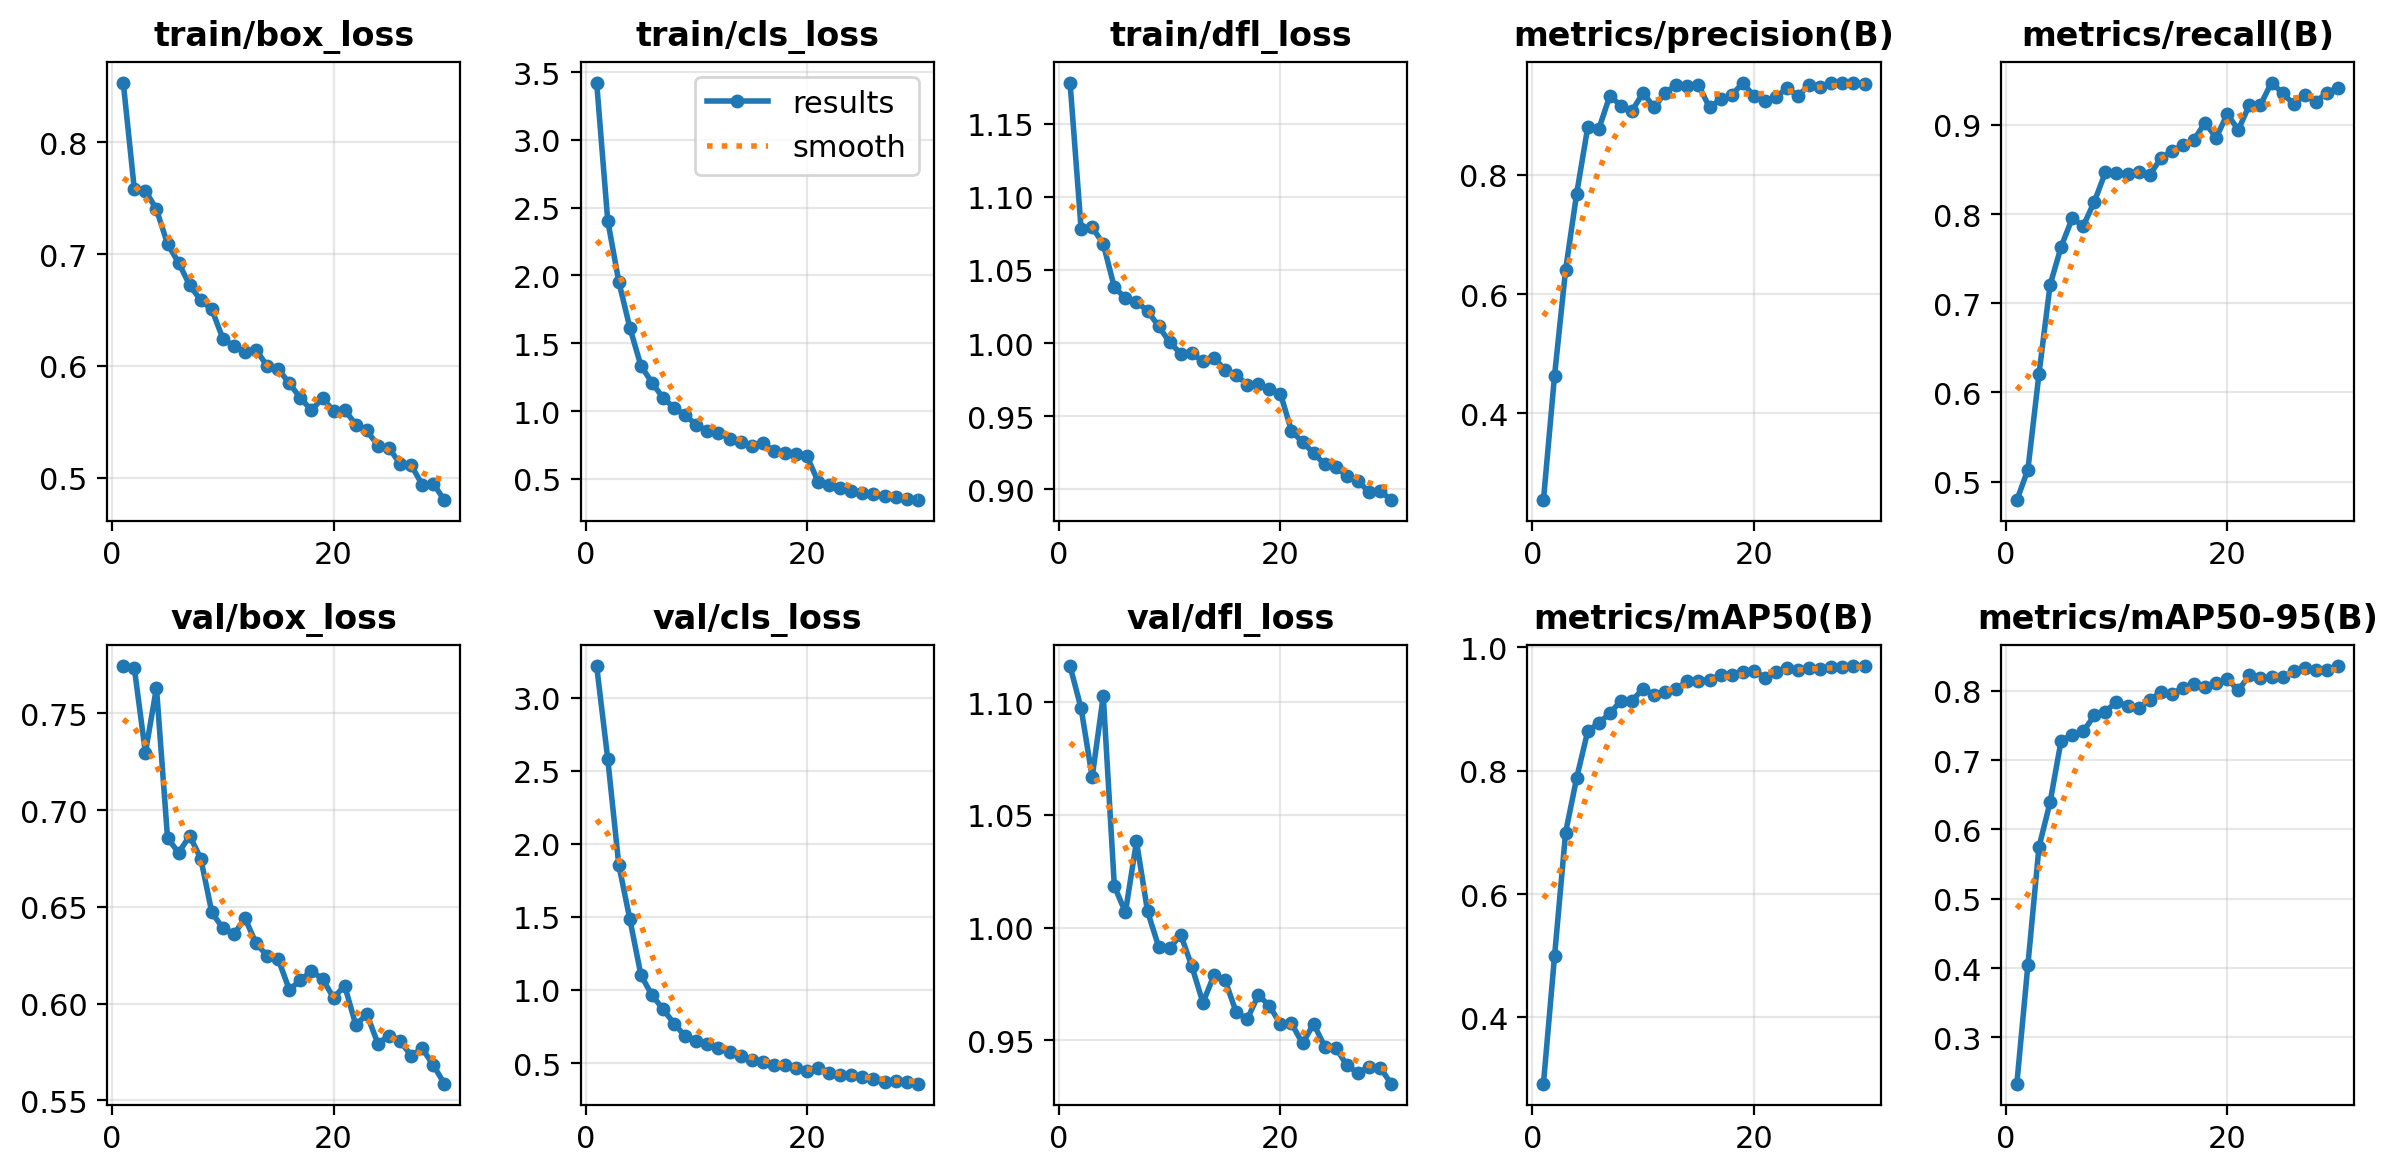
\includegraphics[width=0.95\textwidth]{figures/yolo_training_curves.png}
\caption{Diễn biến hàm mất mát và các chỉ số của YOLOv8n qua 30 chu kỳ huấn luyện}
\label{fig:yolo_curves}
\end{figure}

Hình~\ref{fig:yolo_curves} cho thấy quá trình huấn luyện diễn ra lành mạnh: cả ba thành phần mất
mát đều giảm đơn điệu, mất mát trên tập kiểm định không tách rời khỏi mất mát huấn luyện, và các
chỉ số bão hoà dần từ khoảng chu kỳ thứ 20. Chỉ số trên tập kiểm định ở chu kỳ cuối đạt mAP@0,5
bằng 0,9695 và mAP@0,5:0,95 bằng 0,8354. Khoảng cách giữa con số này và con số trên tập kiểm tra
(0,9539 và 0,8058) là nhỏ và theo đúng chiều mong đợi, cho thấy mô hình không bị quá khớp nghiêm
trọng.

\begin{figure}[H]
\centering
\begin{subfigure}[b]{0.48\textwidth}
  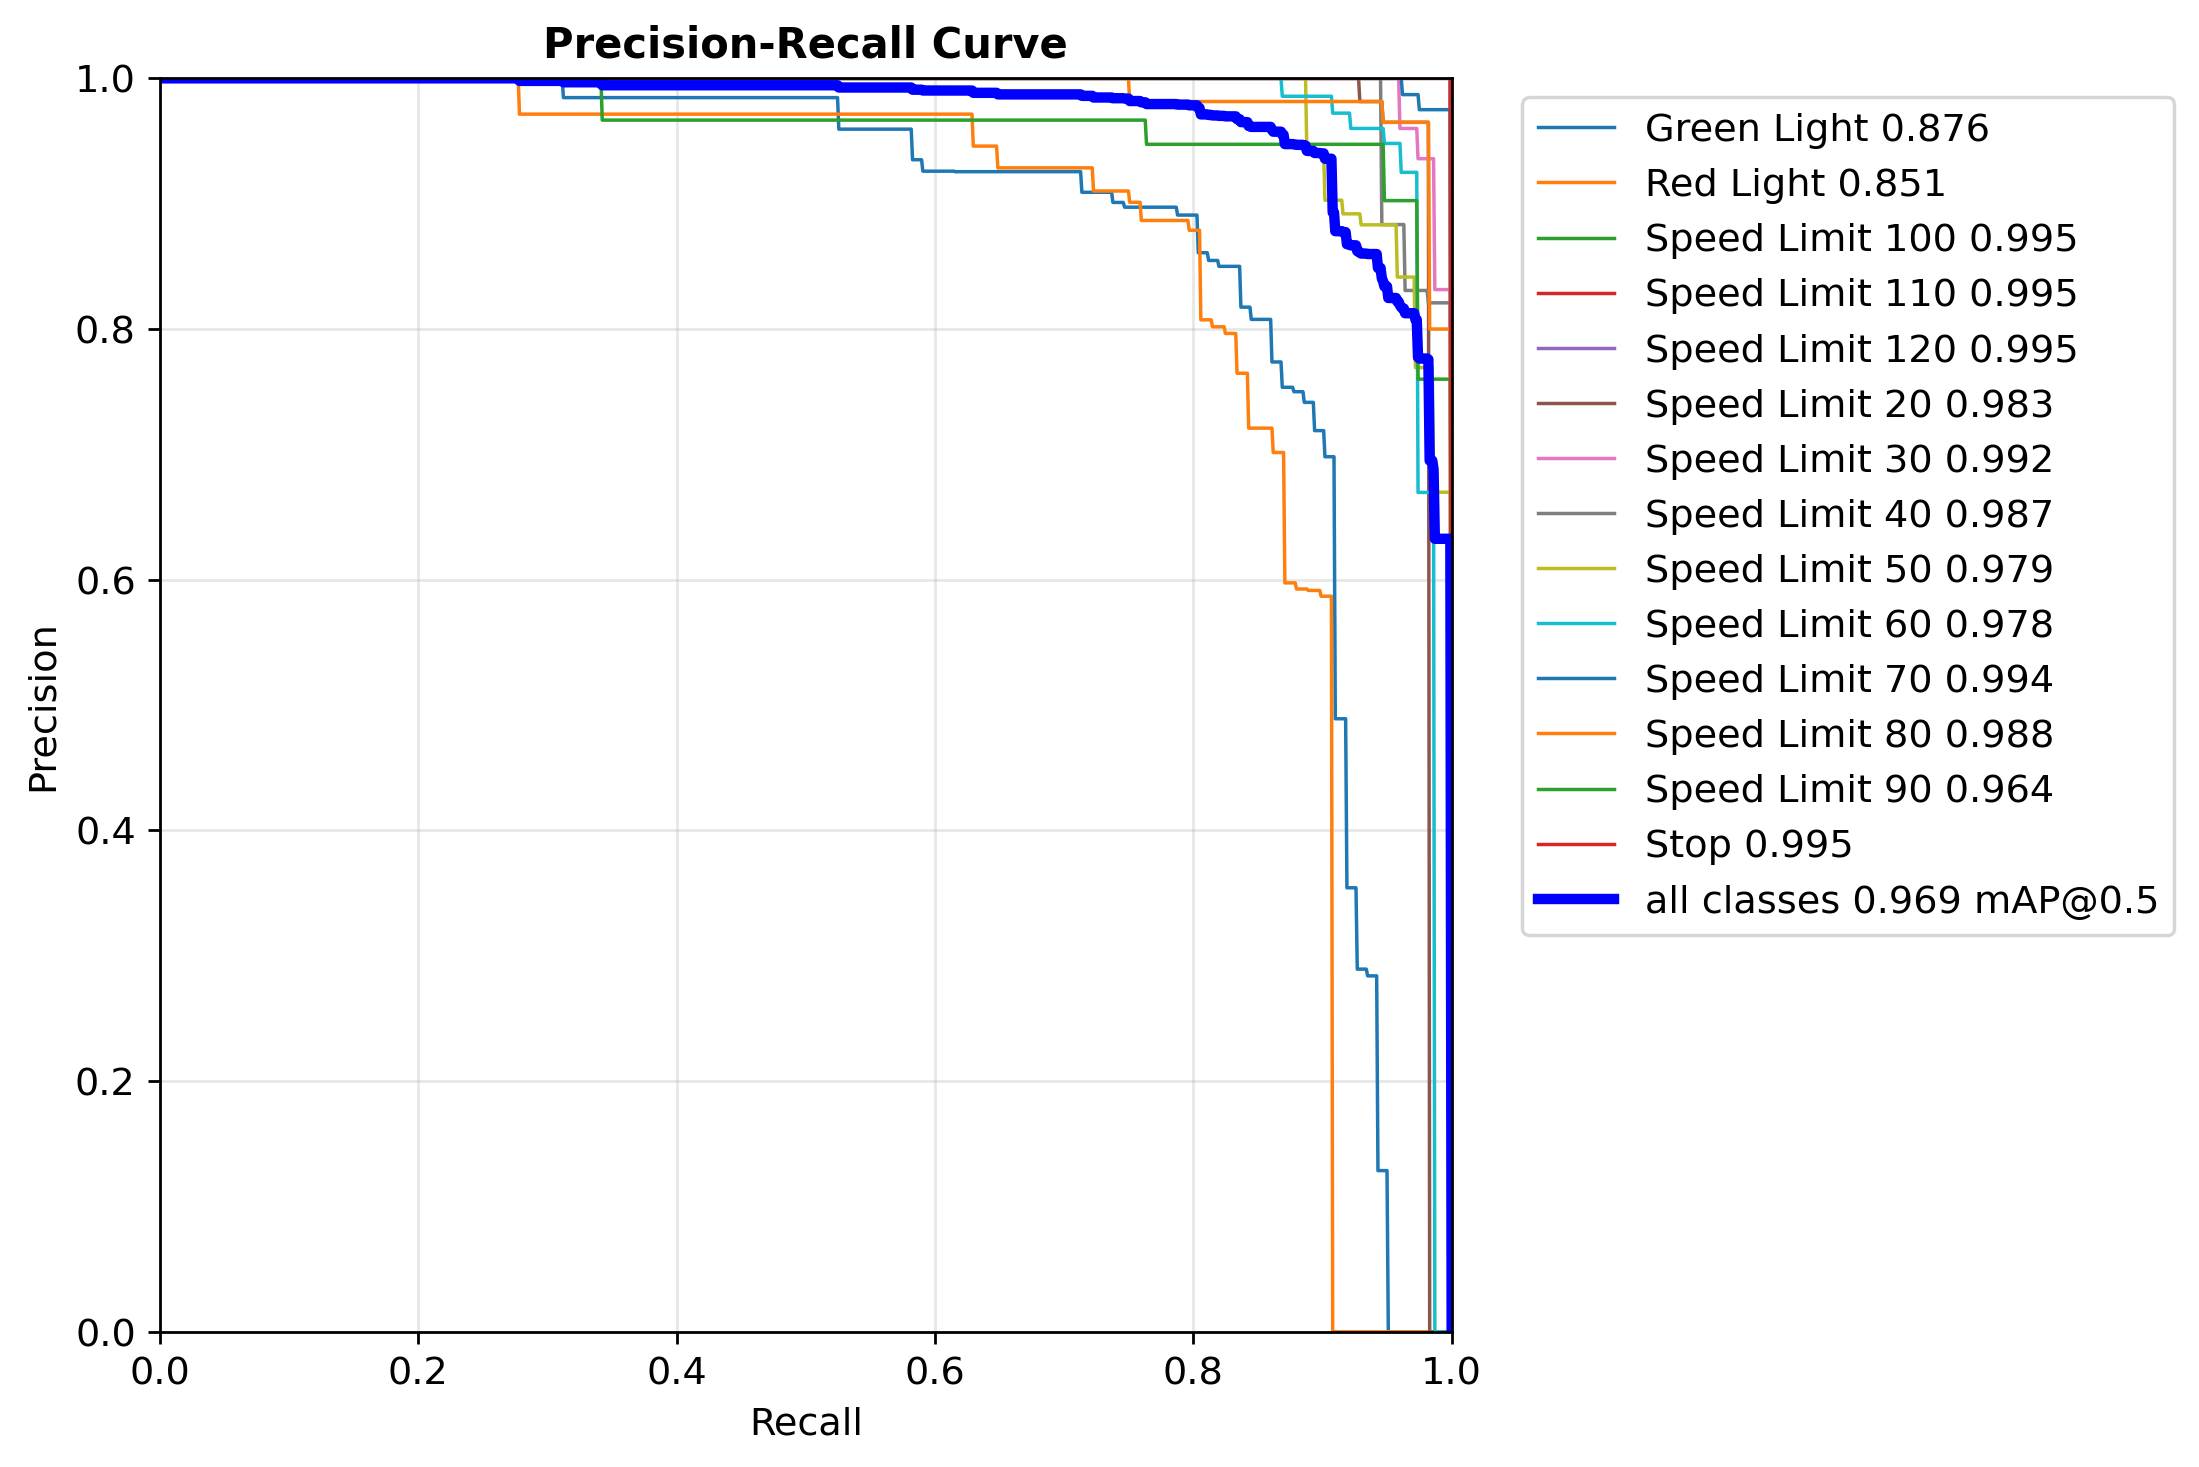
\includegraphics[width=\textwidth]{figures/yolo_pr_curve.png}
  \caption{Đường cong Precision--Recall}
\end{subfigure}
\hfill
\begin{subfigure}[b]{0.48\textwidth}
  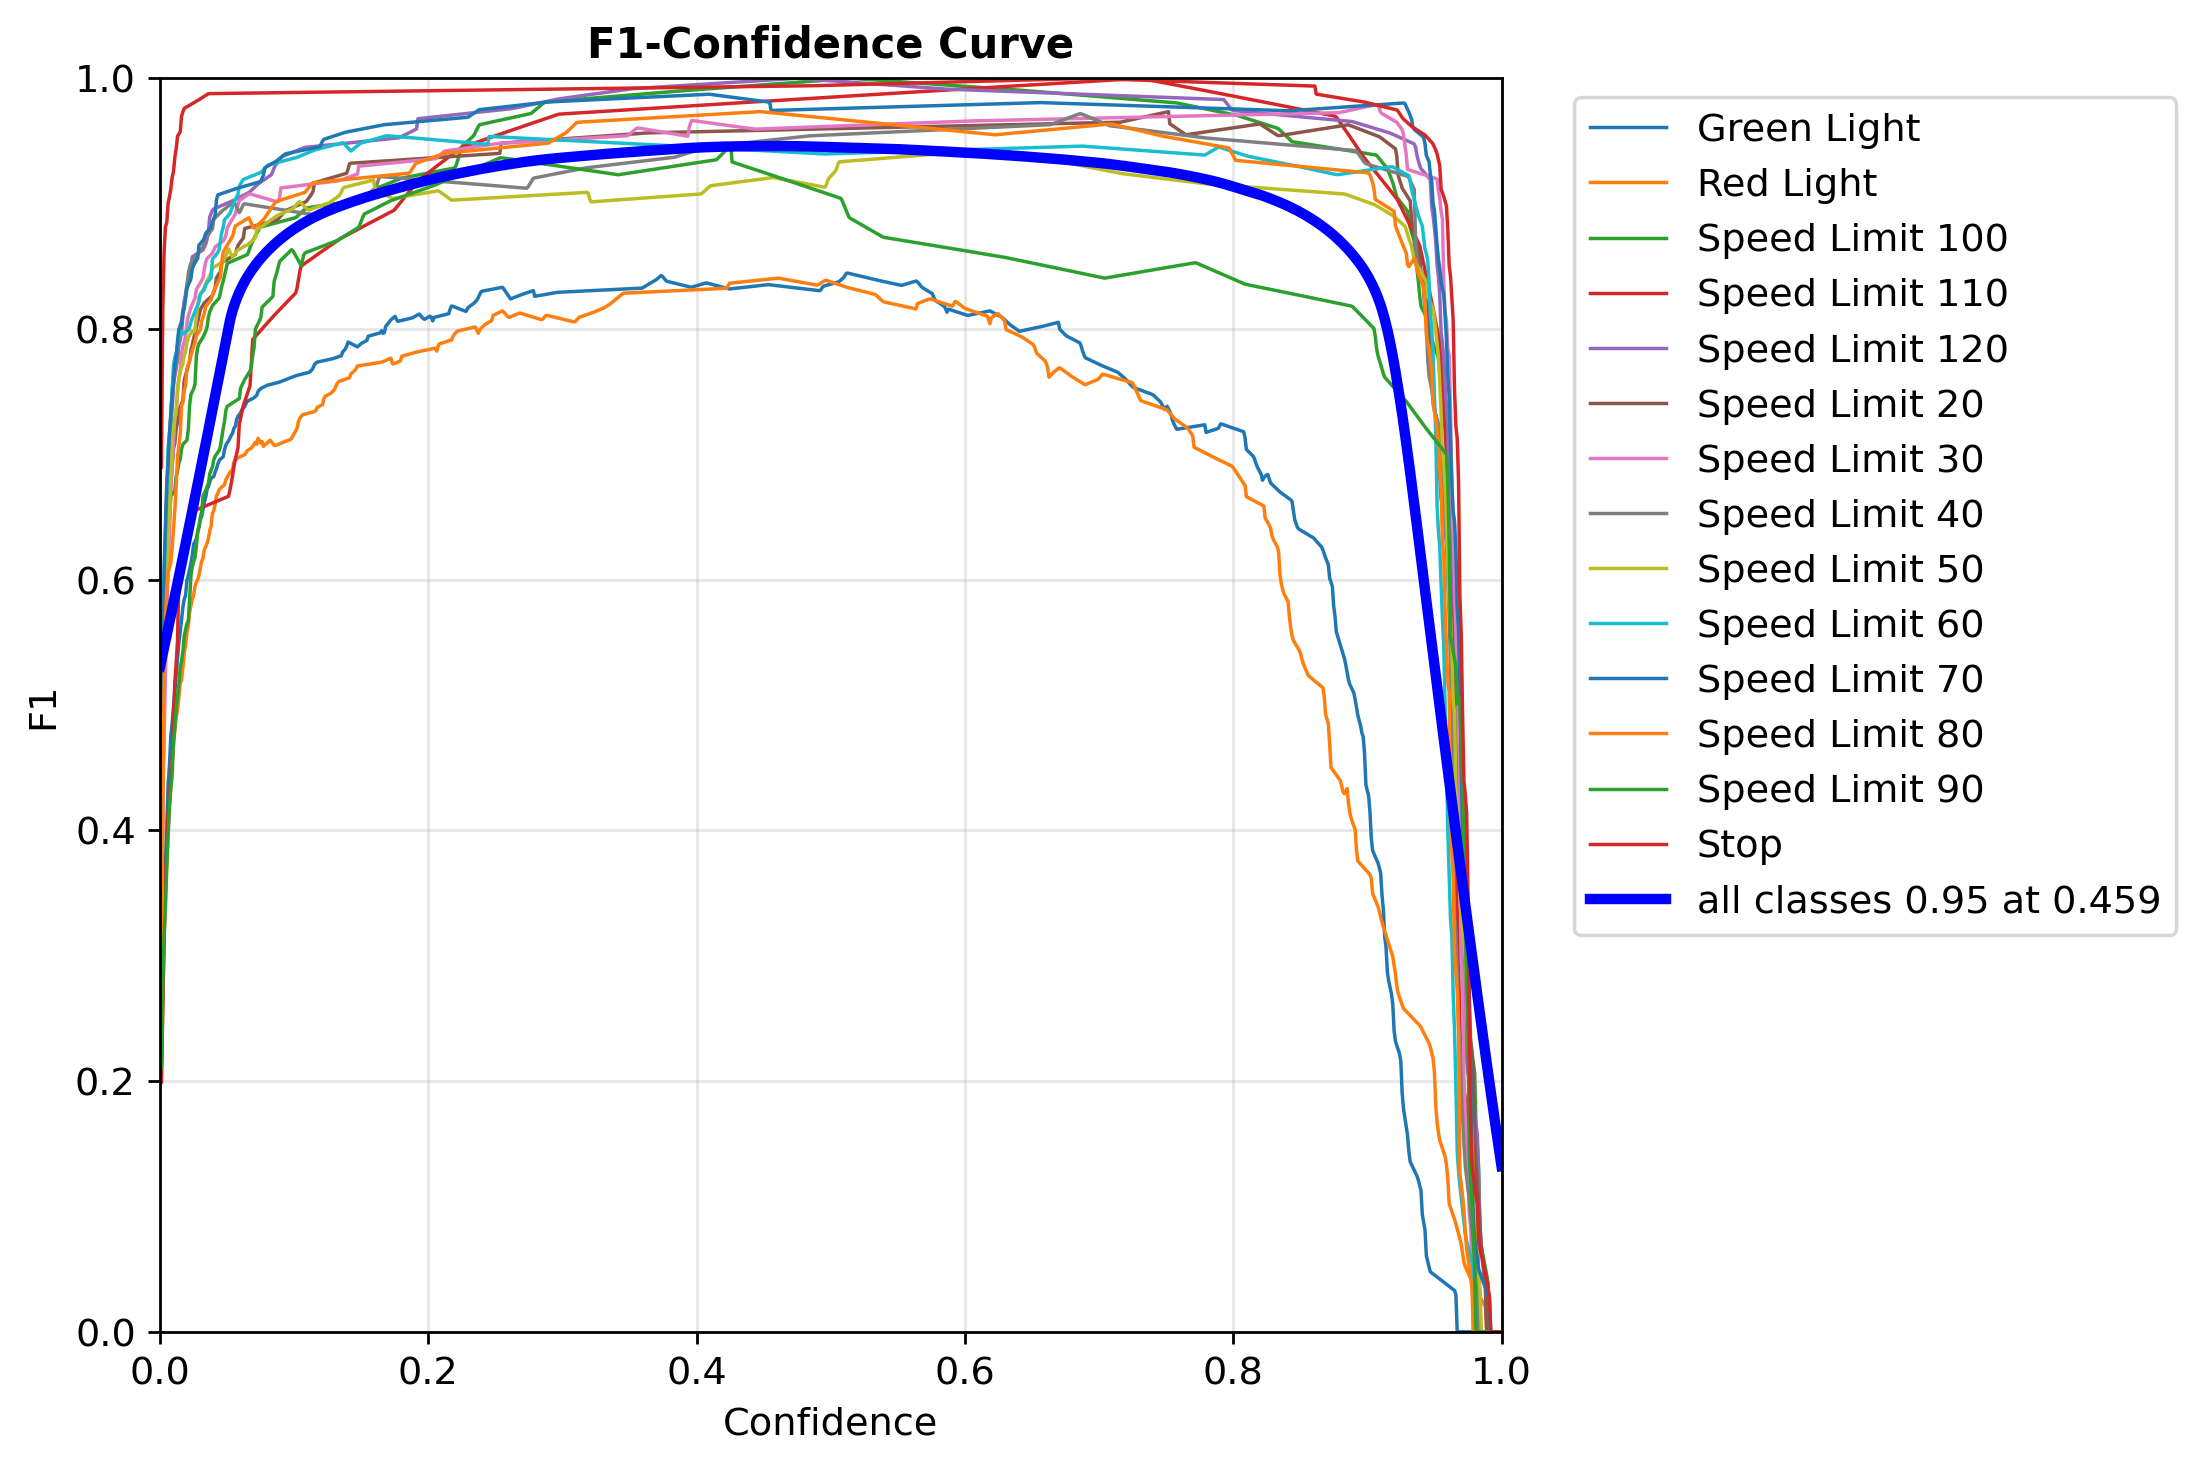
\includegraphics[width=\textwidth]{figures/yolo_f1_curve.png}
  \caption{Đường cong $F_1$ theo ngưỡng tin cậy}
\end{subfigure}
\caption{Đặc tính phân loại của YOLOv8n trên tập kiểm định}
\label{fig:pr_f1}
\end{figure}

\subsection{Vì sao DETR kém hơn tới gần tám lần}
\label{sec:vi_sao_detr}

Chênh lệch giữa 0,9539 và 0,1220 lớn tới mức không thể quy cho một nguyên nhân đơn lẻ. Phân tích
cho thấy có ít nhất năm yếu tố cùng tác động, và \emph{không yếu tố nào trong số đó là bằng chứng
cho thấy kiến trúc transformer kém hơn về bản chất}.

\begin{enumerate}[leftmargin=1.5cm]
\item \textbf{Ngân sách huấn luyện chênh lệch ba lần.} YOLO được huấn luyện 30 chu kỳ, DETR chỉ 10.

\item \textbf{Tốc độ hội tụ đặc thù của DETR.} Bản gốc cần khoảng 300 đến 500 chu kỳ trên
COCO~\cite{carion2020detr}. Với 10 chu kỳ, mô hình về cơ bản vẫn đang ở giai đoạn đầu của quá
trình học phép gán Hungarian.

\item \textbf{Kích thước lô quá nhỏ.} Lô 2 ảnh, bị giới hạn bởi bộ nhớ card đồ hoạ, khiến ước
lượng gradient nhiễu và phép ghép cặp song ánh dao động mạnh giữa các bước.

\item \textbf{Tốc độ học bị hạ để đổi lấy ổn định.} Việc hạ một bậc so với công thức gốc là cần
thiết để tránh phân kỳ, nhưng cái giá là học chậm hơn nhiều.

\item \textbf{Tăng cường dữ liệu hoàn toàn bất đối xứng.} Đây là yếu tố ít được nhắc tới nhất
nhưng có thể là yếu tố nặng ký nhất. Nhánh YOLO nhận đầy đủ bộ tăng cường của Ultralytics gồm ghép
ảnh mosaic hệ số 1,0, biến đổi tỉ lệ 0,5, tịnh tiến 0,1, nhiễu màu HSV và xoá ngẫu nhiên 0,4. Nhánh
DETR \emph{không có bất kỳ phép tăng cường nào} --- bộ dữ liệu chỉ gọi bộ tiền xử lý ảnh rồi trả
về. Với một kiến trúc vốn đã đói dữ liệu~\cite{dosovitskiy2021vit}, việc bị tước toàn bộ tăng
cường là bất lợi rất lớn.
\end{enumerate}

Thêm vào đó, kiến trúc transformer thiếu thiên kiến quy nạp về tính địa phương và bất biến tịnh
tiến vốn có sẵn trong mạng tích chập. Trên một bộ dữ liệu chỉ 6.012 hộp bao, sự thiếu vắng này trở
thành bất lợi rõ rệt. Kết luận đúng đắn rút ra từ E0 vì vậy không phải ``DETR kém hơn YOLO'' mà là
``ở ngân sách dữ liệu và tính toán của đề tài này, YOLO hiệu quả hơn hẳn, còn DETR mới chỉ ở trạng
thái chưa huấn luyện đủ''. Các công trình gần đây như RT-DETR~\cite{zhao2024rtdetr} cho thấy khi
được huấn luyện đầy đủ, dòng transformer hoàn toàn có thể vượt YOLO.

\section{E1 --- Khảo sát kiến trúc nhẹ}

Ba kiến trúc thay thế được thử với kỳ vọng tìm ra phương án nhẹ hơn mà không kém hơn. Cả ba đều
không đạt kỳ vọng.

Mọi con số trong mục này thuộc giai đoạn 2, nên được so với mốc tham chiếu YOLOv8n FP32 của chính
giai đoạn đó (0,9633) chứ không so với con số ở Bảng~\ref{tab:e0}.

YOLO11n, thuộc thế hệ mới hơn YOLOv8n, đạt mAP@0,5 bằng 0,9252 --- thấp hơn mốc tham chiếu 3,81
điểm phần trăm, đồng thời chậm hơn. Đây là kết quả tốt nhất trong nhóm E1 nhưng vẫn không đủ để
thay thế.

SSDLite-MobileNetV3~\cite{liu2016ssd,howard2019mobilenetv3} cho kết quả thấp nhất nhóm với 0,7432.
Đáng chú ý hơn là khoảng cách giữa hai độ đo: mAP@0,5:0,95 chỉ đạt 0,6260, tức mô hình định vị hộp
bao kém khít. Điều này phù hợp với đặc điểm kiến trúc: SSDLite chạy ở độ phân giải đầu vào chỉ 320
điểm ảnh và dùng xương sống rất nhẹ, nên gần như mù với vật thể nhỏ --- vốn chiếm 35,30\% số hộp
bao trong bộ dữ liệu này.

D-FINE-Nano đạt 0,7836, tốt hơn SSDLite về định vị nhưng yếu hơn về phân loại. Điểm đáng ghi nhận
là nó cho thấy một kiến trúc transformer \emph{được thiết kế để hội tụ nhanh} có thể đạt mức chấp
nhận được trong cùng ngân sách mà DETR gốc chỉ đạt 0,1220 --- một xác nhận gián tiếp cho lập luận
ở Mục~\ref{sec:vi_sao_detr} rằng vấn đề của DETR nằm ở tốc độ hội tụ chứ không ở kiến trúc
transformer nói chung.

\section{E2 --- Lượng tử hoá sau huấn luyện}

\begin{table}[H]
\centering
\caption{Ảnh hưởng của lượng tử hoá tới độ chính xác và tốc độ (toàn bộ thuộc giai đoạn 2)}
\label{tab:e2}
\small
\begin{tabular}{lrrrl}
\toprule
\textbf{Cấu hình} & \textbf{mAP@0,5} & \textbf{$\Delta$ so với gốc} & \textbf{FPS} & \textbf{Nhận xét} \\
\midrule
PyTorch FP32 (gốc) & 0,9633 & ---      & 65,3 & Mốc so sánh giai đoạn 2 \\
PyTorch FP16       & 0,9633 & $0{,}0000$   & 65,3 & Không mất độ chính xác \\
ONNX INT8          & 0,9552 & $-0{,}0081$  & 5,7  & Nén tốt nhất, chậm nhất \\
OpenVINO INT8      & 0,9265 & $-0{,}0368$  & 13,9 & Nhanh hơn ONNX INT8 \\
\bottomrule
\end{tabular}
\end{table}

FP16 giữ nguyên hoàn toàn độ chính xác trong khi giảm khoảng một nửa dung lượng --- kết quả phù
hợp với các nghiên cứu về huấn luyện độ chính xác hỗn hợp~\cite{micikevicius2018mixedprecision}.
Đây là lựa chọn không có nhược điểm trong bối cảnh này.

Kết quả INT8 thì trái với kỳ vọng thông thường. Về lý thuyết, biểu diễn số nguyên 8 bit cho phép
dùng các nhân tính toán số nguyên nhanh hơn~\cite{jacob2018quantization}. Trên thực tế, ONNX INT8
chỉ đạt 5,7 khung hình mỗi giây, tức chậm hơn bản FP32 hơn mười một lần. Nguyên nhân nhiều khả
năng là môi trường thực thi CPU dùng trong thí nghiệm không có nhân số nguyên được tối ưu cho mẫu
tính toán của mô hình, nên phần lớn thời gian bị tiêu vào các phép chuyển đổi lượng tử hoá và giải
lượng tử hoá xen giữa các lớp. OpenVINO INT8 nhanh hơn ONNX INT8 khoảng 2,4 lần nhưng đánh đổi
3,68 điểm phần trăm mAP.

Đáng chú ý hơn con số tổng: phần suy giảm do lượng tử hoá INT8 \textbf{tập trung vào nhóm vật thể
nhỏ}. Nhóm E2 không đo $AP$ tách theo kích thước nên không định lượng được trực tiếp, nhưng nhóm E3
--- vốn có thí nghiệm lượng tử hoá riêng và được đo bằng pycocotools --- cho con số cụ thể: khi
chuyển từ ONNX FP32 sang ONNX INT8, mAP@0,5 chỉ giảm 0,0038 trong khi $AP$ trên vật thể nhỏ giảm
0,0247, tức \textbf{gấp 6,5 lần} (xem Bảng~\ref{tab:e3_delta}).

Điều này hợp lý về mặt cơ chế: lượng tử hoá làm giảm độ phân giải biểu diễn của các giá trị kích
hoạt, và vật thể nhỏ vốn đã cho tín hiệu yếu trên bản đồ đặc trưng nên chịu thiệt nhiều nhất. Hệ
quả thực tiễn rất cụ thể: với bài toán biển báo giao thông, nơi 35,30\% hộp bao thuộc nhóm nhỏ và
biển ở xa mới là trường hợp quan trọng, một cấu hình INT8 nhìn qua ``chỉ mất vài phần nghìn mAP''
có thể mất nhiều hơn hẳn ở đúng nhóm cần quan tâm. Khi chọn cấu hình triển khai, phải đọc $AP$ tách
theo nhóm kích thước chứ không chỉ đọc mAP tổng.

\hopnhanmanh{Bài học rút ra là lượng tử hoá INT8 không tự động đồng nghĩa với suy luận nhanh hơn;
lợi ích của nó phụ thuộc chặt vào môi trường thực thi và phần cứng đích. Trong bối cảnh của đề
tài, FP16 là lựa chọn hợp lý duy nhất.}

\section{Kết quả trái với kỳ vọng}
\label{sec:trai_ky_vong}

\subsection{E3 --- Chưng cất tri thức cho kết quả âm}

Giả thuyết ban đầu là mô hình học trò YOLO26n sẽ hưởng lợi từ phân phối đầu ra mềm của mô hình
thầy YOLO26s~\cite{hinton2015distillation}. Kết quả ngược lại.

Khác với các nhóm còn lại, nhóm E3 được đánh giá bằng \textbf{pycocotools} trên tệp chú thích COCO
của tập kiểm tra, nên ngoài mAP tổng còn có $AP$ tách theo nhóm kích thước. Bảng~\ref{tab:e3} trình
bày đầy đủ, bao gồm cả hai cấu hình xuất sang ONNX của chính mô hình chưng cất.

\begin{table}[H]
\centering
\caption{Kết quả nhóm E3 đo bằng pycocotools trên tập kiểm tra}
\label{tab:e3}
\footnotesize
\begin{tabular}{lrrrrrrr}
\toprule
\textbf{Cấu hình} & \textbf{Tham số (M)} & \textbf{Tệp (MB)} & \textbf{mAP@0,5} & \textbf{mAP@.5:.95} & \textbf{$AP$ nhỏ} & \textbf{$AP$ lớn} & \textbf{FPS} \\
\midrule
YOLO26s (thầy)        & 9,47 & 19,39 & 0,9520 & 0,7822 & 0,616 & 0,859 & 74,4 \\
YOLO26n đối chứng     & 2,38 & 5,15  & \textbf{0,9348} & \textbf{0,7773} & \textbf{0,548} & \textbf{0,862} & 69,7 \\
YOLO26n chưng cất     & 2,38 & 5,15  & 0,9014 & 0,7450 & 0,486 & 0,852 & 74,8 \\
\midrule
ONNX FP32 (từ trò KD) & ---  & 9,35  & 0,9079 & 0,7473 & 0,462 & 0,847 & 19,8 \\
ONNX INT8 (từ trò KD) & ---  & 2,78  & 0,9041 & 0,7437 & 0,437 & 0,839 & 9,4 \\
\bottomrule
\end{tabular}
\end{table}

\subsubsection*{Chưng cất thực sự đã được kích hoạt}

Trước khi diễn giải một kết quả âm, cần loại trừ khả năng cơ chế chưng cất không hề chạy. Nhật ký
huấn luyện của nhánh chưng cất có thêm cột \texttt{train/dis\_loss} --- cột này không tồn tại ở
nhánh đối chứng --- và giá trị của nó giảm từ 12,1663 ở chu kỳ đầu xuống 1,1608 ở chu kỳ cuối. Hàm
mất mát chưng cất đã hoạt động và đã hội tụ; kết quả âm là kết quả thật chứ không phải lỗi cấu hình.

\subsubsection*{Suy giảm tập trung ở vật thể nhỏ}

\begin{table}[H]
\centering
\caption{Ba phép so sánh cốt lõi của nhóm E3}
\label{tab:e3_delta}
\small
\begin{tabular}{lrrr}
\toprule
\textbf{Phép so sánh} & \textbf{$\Delta$ mAP@0,5} & \textbf{$\Delta$ mAP@.5:.95} & \textbf{$\Delta$ $AP$ nhỏ} \\
\midrule
Trò chưng cất so với trò đối chứng & $-0{,}0334$ & $-0{,}0323$ & $\mathbf{-0{,}0620}$ \\
Trò chưng cất so với thầy          & $-0{,}0507$ & $-0{,}0372$ & $\mathbf{-0{,}1308}$ \\
ONNX INT8 so với ONNX FP32         & $-0{,}0038$ & $-0{,}0036$ & $\mathbf{-0{,}0247}$ \\
\bottomrule
\end{tabular}
\end{table}

\hopnhanmanh{Cột $AP$ nhỏ là cột đáng đọc nhất. Ở cả ba phép so sánh, mức suy giảm trên vật thể nhỏ
đều lớn hơn mức suy giảm trên mAP tổng --- gấp 1,9 lần ở phép chưng cất và gấp \textbf{6,5 lần} ở
phép lượng tử hoá INT8. Một cấu hình nhìn qua chỉ ``mất 0,38 điểm mAP'' thực chất mất 2,47 điểm ở
đúng nhóm vật thể quan trọng nhất đối với bài toán biển báo giao thông.}

Cột $AP$ lớn cho thấy điều ngược lại: cả ba mô hình PyTorch đều nằm quanh mức 0,85--0,86, gần như
không phân biệt được. Nói cách khác, mọi khác biệt giữa các cấu hình đều nằm ở vật thể nhỏ, còn với
vật thể lớn thì bài toán đã bão hoà. Điều này nhất quán với phân tích thành phần bộ dữ liệu ở
Mục~\ref{sec:thanhphan}: hơn một nửa số hộp bao thuộc nhóm lớn và chúng quá dễ để tạo ra khác biệt
giữa các mô hình.

\subsubsection*{Vì sao chưng cất thất bại}

Mô hình được chưng cất thấp hơn đối chứng 3,34 điểm phần trăm mAP@0,5 và 6,20 điểm phần trăm $AP$
trên vật thể nhỏ. Có ba cách giải thích khả dĩ. Thứ nhất, khoảng cách năng lực giữa thầy và trò quá
hẹp: thầy chỉ đạt 0,9520, tức nhỉnh hơn trò đối chứng 1,72 điểm phần trăm, nên lượng ``tri thức
tối'' có thể truyền đạt là rất ít --- trong khi chi phí nhiễu do bắt chước một phân phối không hoàn
hảo thì vẫn phải trả đủ. Thứ hai, kích thước lô của nhánh chưng cất chỉ bằng 8 so với 24 của nhánh
đối chứng, do phải nạp đồng thời cả hai mô hình vào bộ nhớ card đồ hoạ; đây là một yếu tố gây nhiễu
chưa được kiểm soát và tự nó đã đủ giải thích một phần chênh lệch. Thứ ba, hệ số chưng cất 6,0 ---
giá trị mặc định của thư viện --- có thể quá lớn với một cặp thầy--trò gần nhau như vậy, khiến
thành phần bắt chước lấn át tín hiệu từ nhãn cứng.

Đáng chú ý, thí nghiệm được thiết kế kèm \emph{ngưỡng chấp nhận khai báo trước khi chạy}. Trong năm
ngưỡng, ba đạt và hai không đạt --- cả hai ngưỡng không đạt đều thuộc về giả thuyết chưng cất. Việc
khai báo tiêu chí trước và báo cáo cả kết quả không đạt là cách làm đúng đắn về mặt phương pháp: nó
ngăn việc diễn giải lại kỳ vọng sau khi đã nhìn thấy số liệu.

\begin{table}[H]
\centering
\caption{Kiểm tra các ngưỡng chấp nhận khai báo trước khi chạy thực nghiệm}
\label{tab:e3_thresh}
\small
\begin{tabular}{lll}
\toprule
\textbf{Ngưỡng} & \textbf{Giá trị đo} & \textbf{Kết quả} \\
\midrule
KD không kém đối chứng quá 0,5 điểm      & $\Delta = -0{,}0323$ & \textbf{KHÔNG ĐẠT} \\
KD tốt hơn đối chứng (kỳ vọng ban đầu)   & $\Delta = -0{,}0323$ & \textbf{KHÔNG ĐẠT} \\
INT8 giảm không quá 1,5 điểm so với FP32 & giảm $0{,}0036$      & ĐẠT \\
INT8 nhỏ hơn FP32 ít nhất 50\%           & giảm 70,3\%          & ĐẠT \\
Trò chưng cất nhẹ hơn thầy               & 5,15 so với 19,39 MB & ĐẠT \\
\bottomrule
\end{tabular}
\end{table}

Kết quả này được giữ lại trong báo cáo thay vì loại bỏ, vì nó xác định rõ \emph{điều kiện áp dụng}
của kỹ thuật: chưng cất tri thức chỉ có ý nghĩa khi tồn tại khoảng cách năng lực đủ lớn giữa thầy và
trò, và khi mô hình thầy thực sự mạnh. Muốn kết luận chắc chắn hơn, cần chạy lại nhánh chưng cất với
cùng kích thước lô như nhánh đối chứng và quét hệ số chưng cất thay vì dùng giá trị mặc định.

\subsection{Khoảng cách giữa chỉ số và hành vi thực tế}

Kết quả trái kỳ vọng thứ hai mang tính hệ thống hơn. Mô hình đạt mAP@0,5 bằng 0,9539 trên tập kiểm
tra, nhưng khi chạy trên video đường phố thực tế thu bằng camera hành trình, khả năng phát hiện
suy giảm rõ rệt, đặc biệt với biển báo ở xa.

Phân tích thành phần bộ dữ liệu ở Mục~\ref{sec:thanhphan} giải thích hiện tượng này. Với 38,68\%
số ảnh huấn luyện là ảnh cắt cận cảnh có cạnh biển chiếm 66,8\% cạnh ảnh, mô hình được dạy rất kỹ
chế độ ``biển lấp đầy khung hình''. Trong khi đó, chế độ thực sự quan trọng khi lái xe --- biển báo
cách 30 đến 50 mét, tương ứng khoảng 30 đến 80 điểm ảnh trong khung hình Full HD --- gần như không
xuất hiện trong dữ liệu, như Bảng~\ref{tab:percentile} đã chỉ ra.

Vấn đề càng nghiêm trọng hơn ở khâu suy luận. Khi một khung hình 1920$\times$1080 được đưa vào mô
hình huấn luyện ở kích thước 640, thư viện sẽ co ảnh theo hệ số khoảng 0,33. Một biển báo 40 điểm
ảnh trở thành 13 điểm ảnh, chỉ trải trên khoảng 1,6 ô lưới của đầu dự đoán P3 vốn hoạt động ở bước
sải 8 --- tức nằm ngay ở giới hạn khả năng phát hiện.

Cần nhấn mạnh rằng \emph{tập kiểm tra không phát hiện được vấn đề này}, bởi nó có cùng phân bố với
tập huấn luyện. Đây chính là dạng thất bại mà tài liệu về thiên lệch bộ dữ liệu đã cảnh
báo~\cite{torralba2011bias,recht2019imagenetv2}: chỉ số cao trên tập kiểm tra cùng phân bố không
bảo đảm năng lực trên dữ liệu thật.

Một yếu tố thứ hai làm chỉ số bị thổi phồng: thủ tục kiểm toán rò rỉ phát hiện \textbf{155 nhóm ảnh
nguồn xuất hiện ở nhiều hơn một tập}, trong đó \textbf{101 nhóm trùng byte hoàn toàn}. Quy về tập
kiểm tra, có \textbf{65 trong số 638 ảnh có bản sao trong tập huấn luyện}, tức 10,2\% bị rò rỉ, chỉ
còn \textbf{573 ảnh thực sự sạch}. Hiện tượng trùng lặp gần giữa các tập là một nguồn sai lệch đã được
ghi nhận trên nhiều bộ chuẩn phổ biến~\cite{barz2020duplicates}: mô hình đã nhìn thấy đúng những
ảnh đó trong lúc huấn luyện, nên phần dự đoán trên chúng thiên về ghi nhớ hơn là khái quát hoá. Con
số 0,9539 vì vậy nên được hiểu là cận trên, và mọi so sánh nghiêm túc về sau nên báo cáo thêm một
cột đo riêng trên 573 ảnh sạch.

\section{Phân tích lỗi}

\subsection{Nhầm lẫn giữa các lớp}

\begin{figure}[H]
\centering
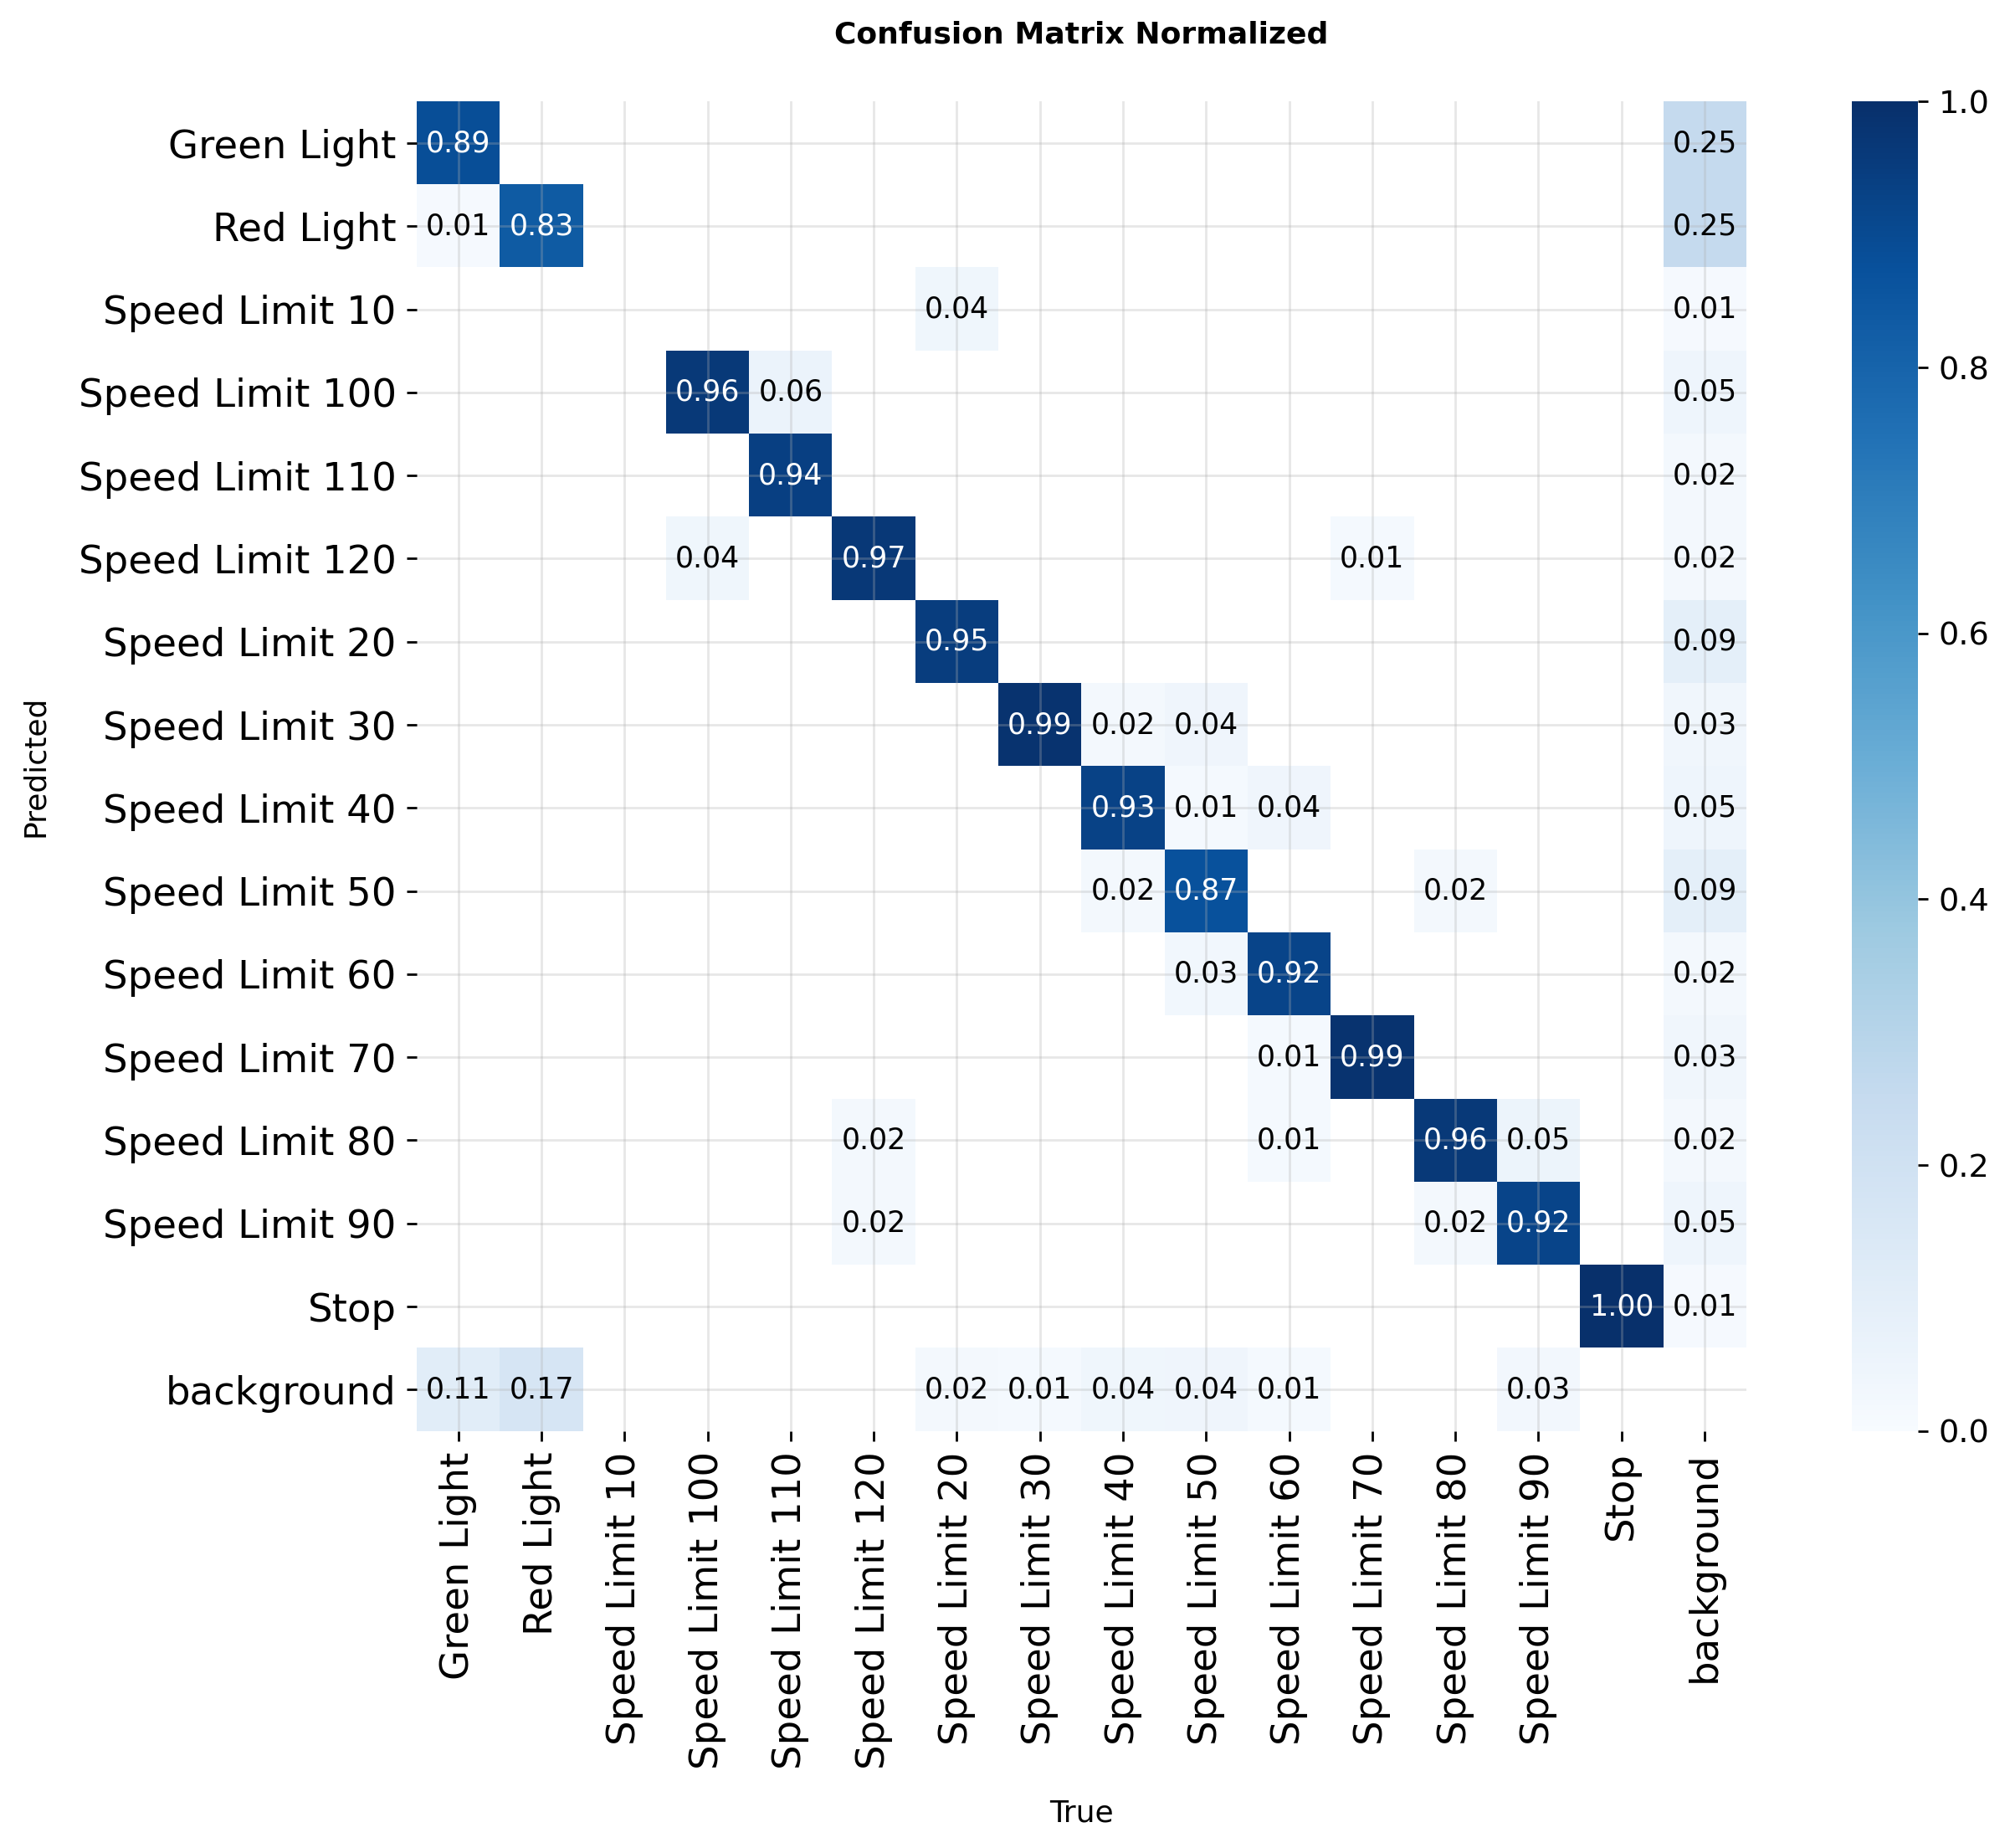
\includegraphics[width=0.88\textwidth]{figures/yolo_confusion_norm.png}
\caption{Ma trận nhầm lẫn chuẩn hoá của YOLOv8n trên tập kiểm định}
\label{fig:confusion}
\end{figure}

Ma trận nhầm lẫn ở Hình~\ref{fig:confusion} cho thấy đường chéo chính chiếm ưu thế rõ rệt. Các
nhầm lẫn còn lại tập trung vào nhóm biển giới hạn tốc độ. Điều này hợp lý về mặt thị giác: mười ba
lớp giới hạn tốc độ có hình dạng, màu sắc và viền hoàn toàn giống nhau, chỉ khác ở chữ số bên
trong. Ở độ phân giải thấp, chữ số là chi tiết đầu tiên bị mất, trong khi hình tròn viền đỏ vẫn
nhận ra được. Nói cách khác, mô hình \emph{định vị} tốt hơn \emph{phân loại}.

Quan sát này gợi ý một hướng thiết kế: tách bài toán thành hai giai đoạn, một bộ phát hiện không
phân biệt lớp để tìm vị trí biển báo, và một bộ phân lớp riêng chạy trên ảnh đã cắt. Cách tổ chức
này cũng cho phép tận dụng đúng mục đích 1.922 ảnh cắt kiểu GTSRB vốn được sinh ra cho bài toán
phân lớp.

\subsection{Ảnh hưởng của mất cân bằng lớp}

Lớp \textit{Speed Limit 10} chỉ có 22 mẫu trên toàn bộ dữ liệu, tương đương khoảng 15 mẫu trong
tập huấn luyện. Với số lượng này, mô hình khó học được biểu diễn ổn định, và bất kỳ chỉ số nào
tính riêng cho lớp đó đều có phương sai rất lớn. Đây là biểu hiện điển hình của bài toán mất cân
bằng lớp trong học sâu~\cite{johnson2019imbalance}.

Cần lưu ý rằng mAP lấy trung bình \emph{không có trọng số} trên các lớp, nên một lớp thiểu số có
$AP$ thấp sẽ kéo mAP tổng xuống ngang bằng với một lớp đa số. Việc mô hình vẫn đạt 0,9539 cho thấy
các lớp thiểu số không quá kém --- nhưng cũng có thể phản ánh việc các mẫu hiếm trong tập kiểm tra
tình cờ dễ.

\begin{figure}[H]
\centering
\begin{subfigure}[b]{0.48\textwidth}
  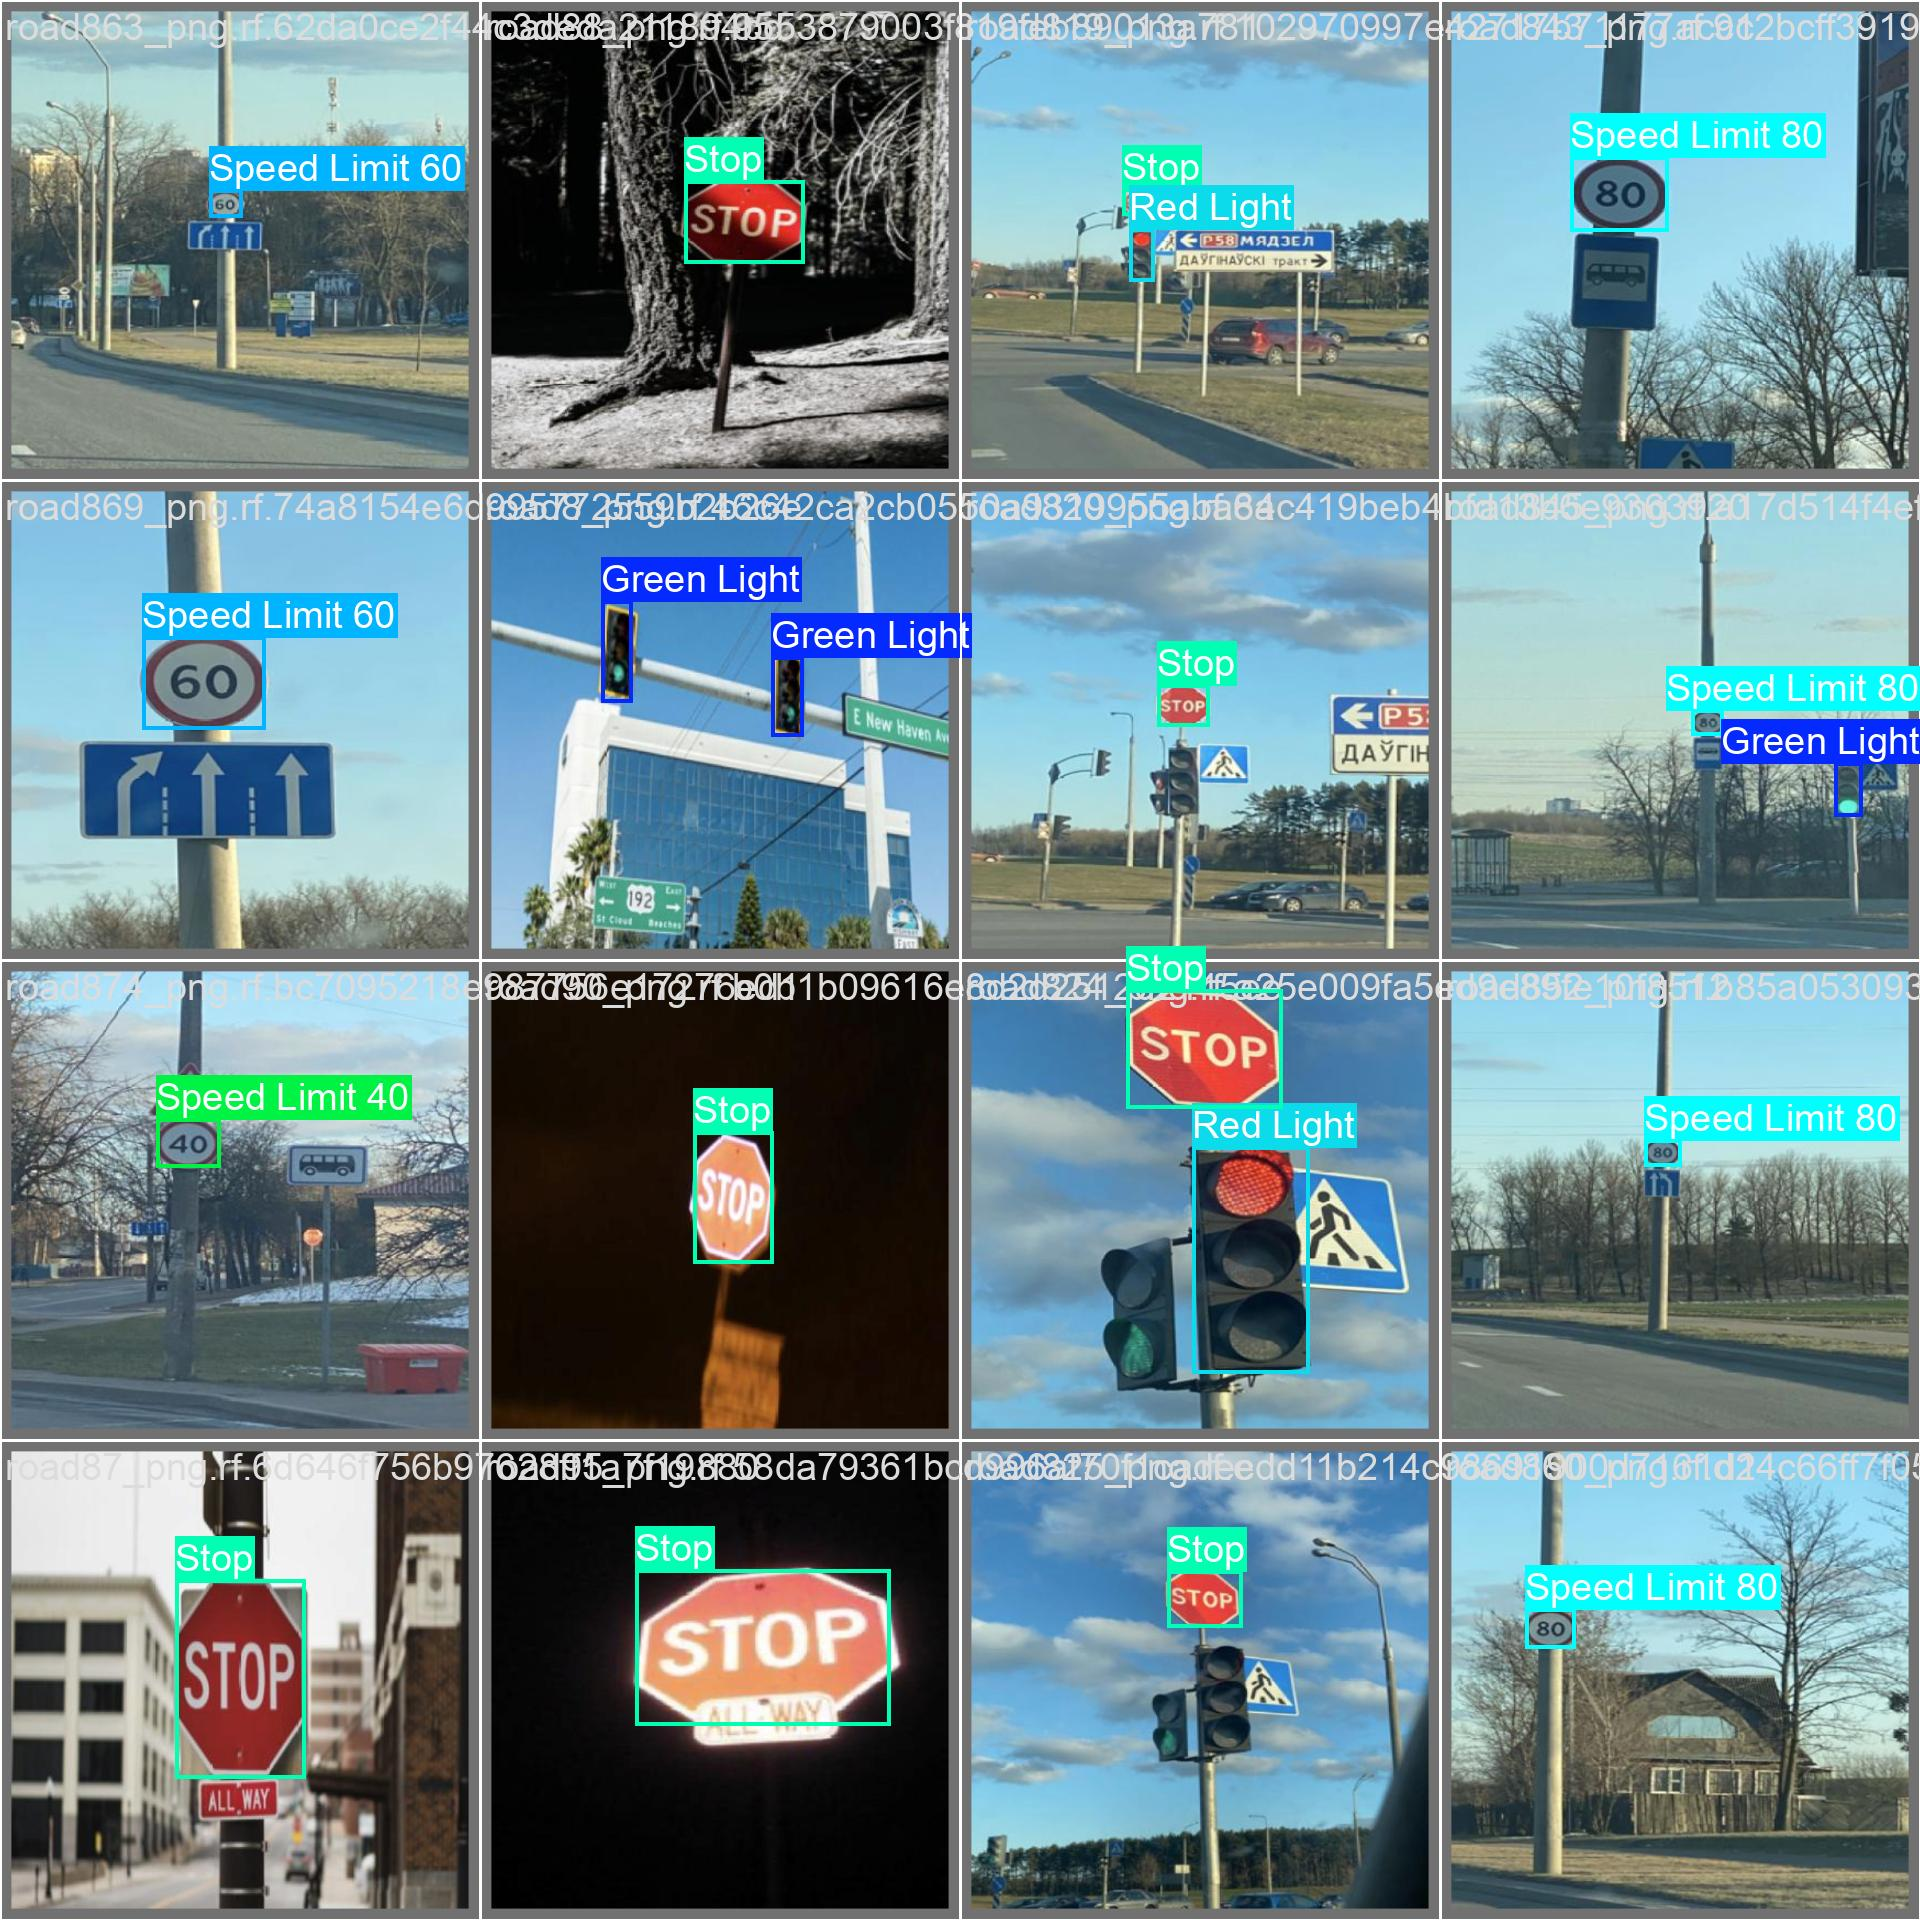
\includegraphics[width=\textwidth]{figures/yolo_val_gt.jpg}
  \caption{Nhãn thật}
\end{subfigure}
\hfill
\begin{subfigure}[b]{0.48\textwidth}
  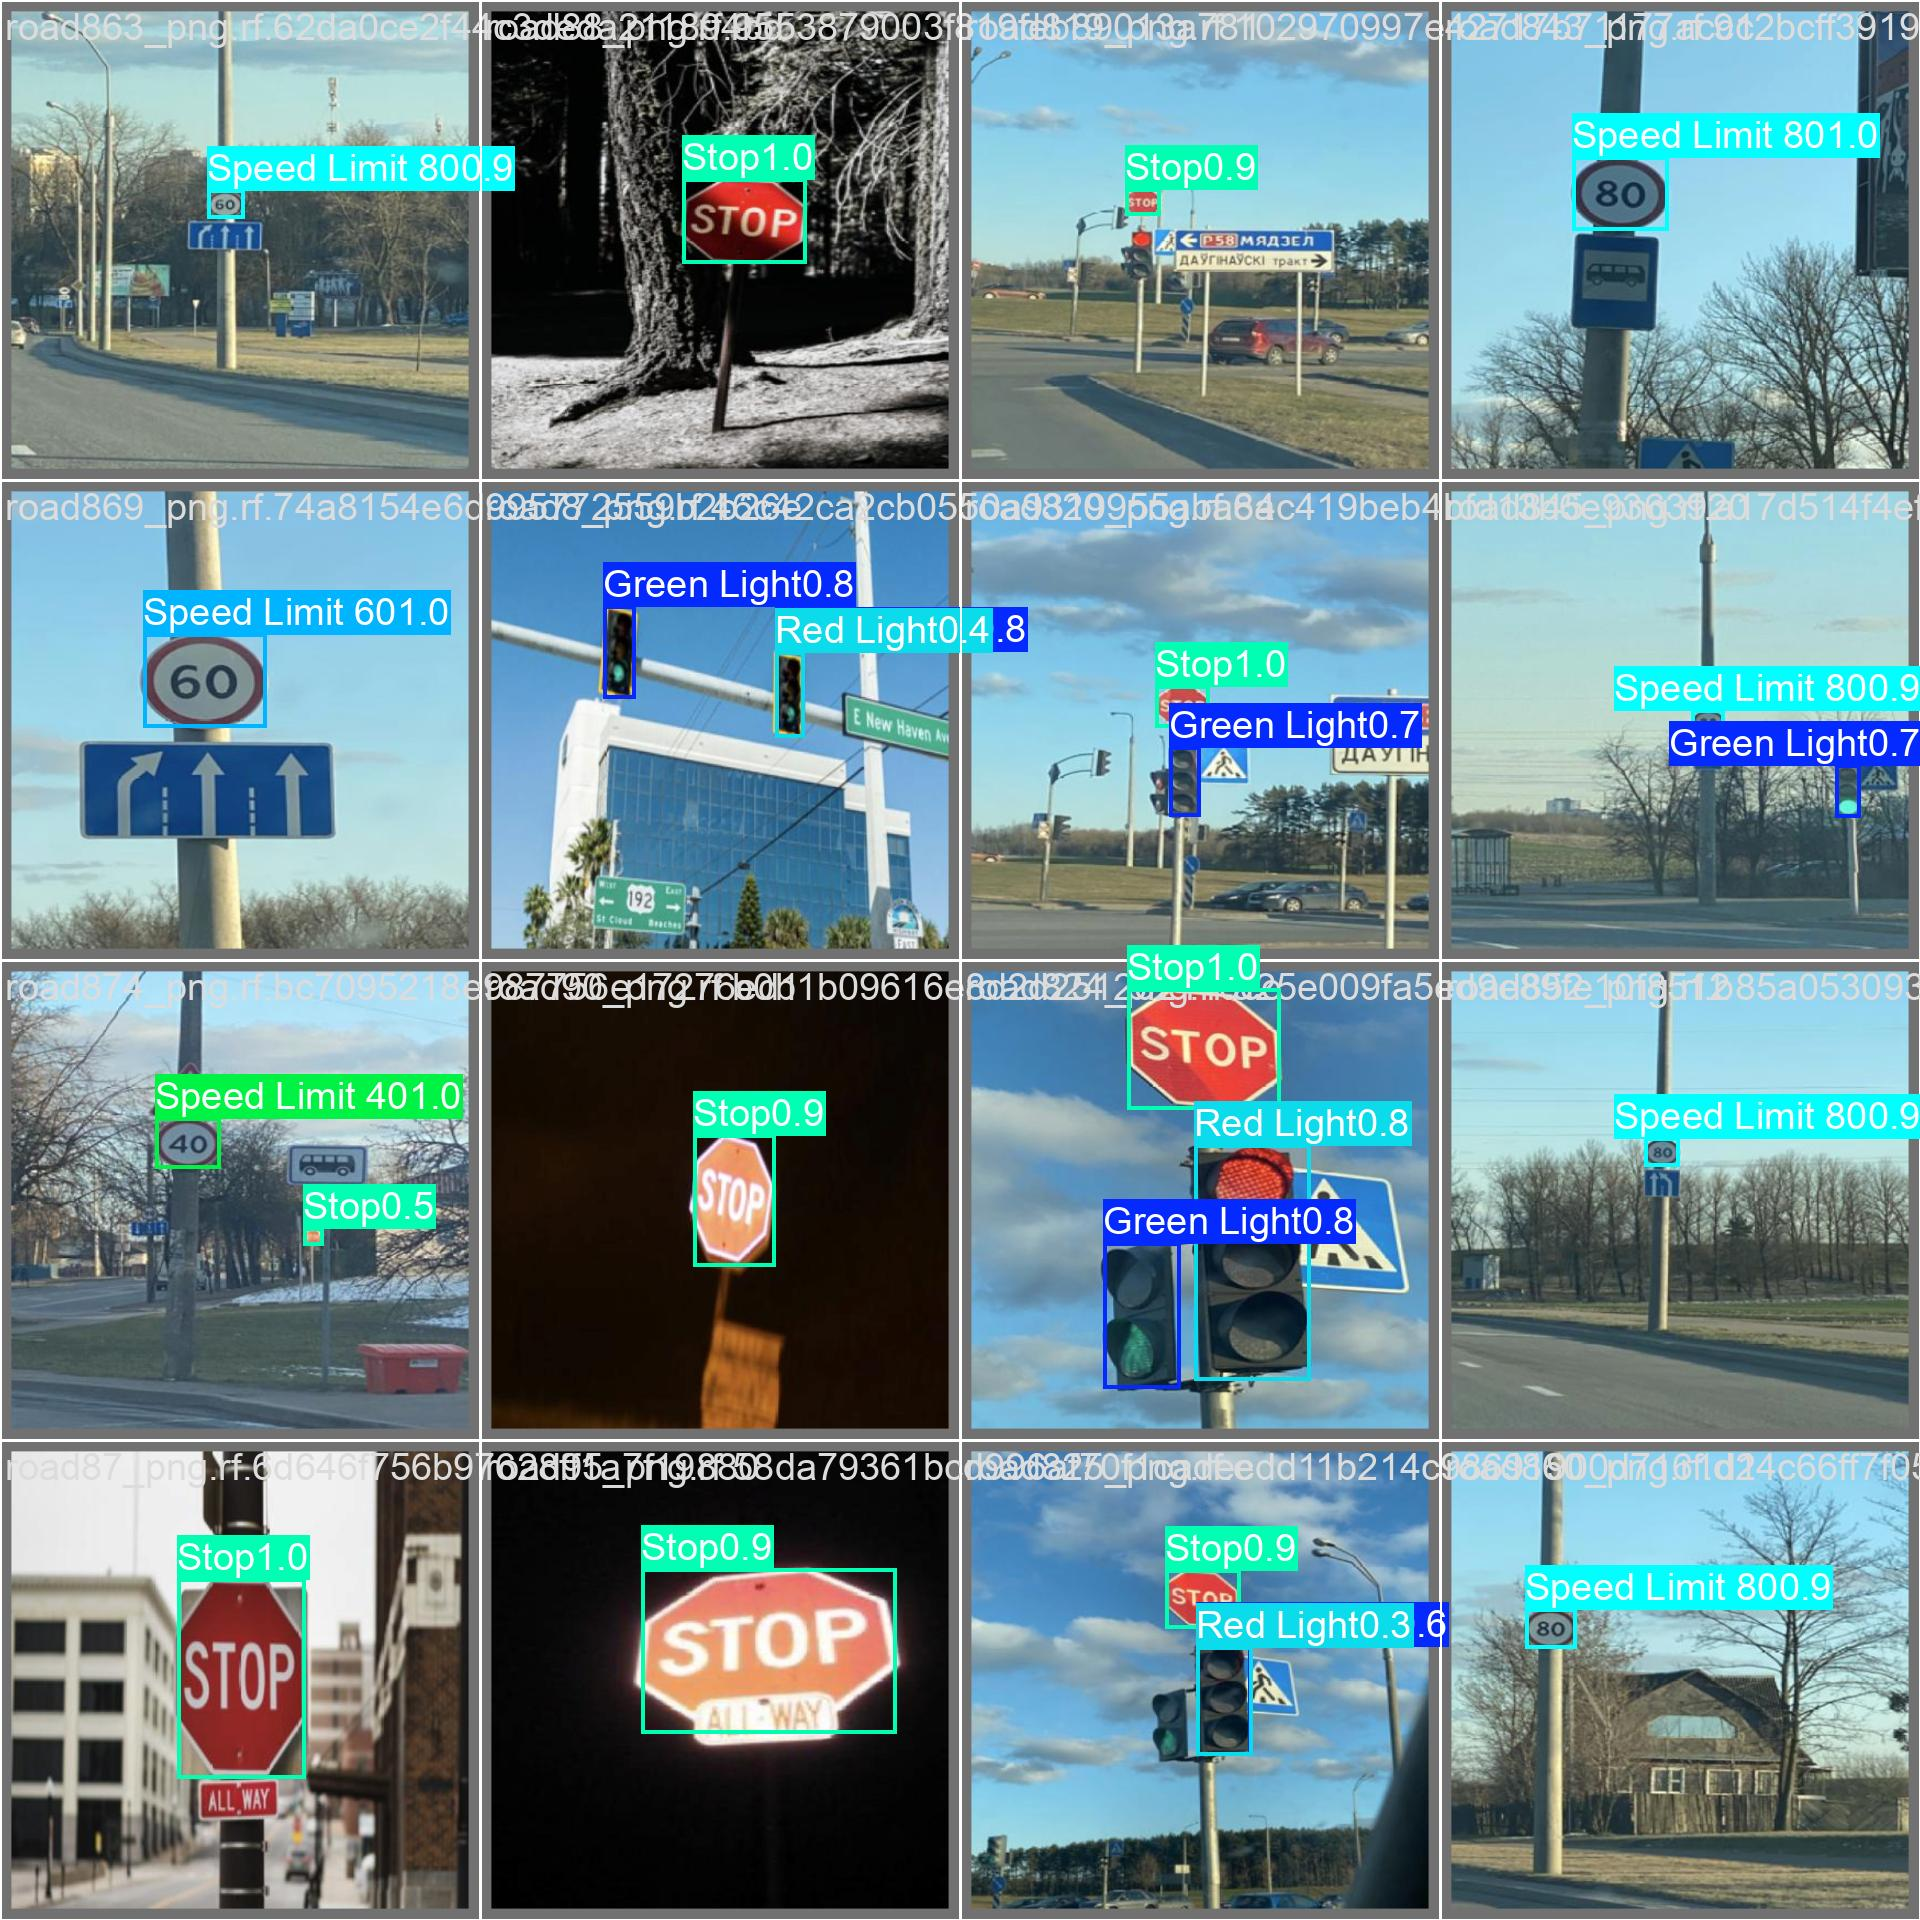
\includegraphics[width=\textwidth]{figures/yolo_val_pred.jpg}
  \caption{Dự đoán của mô hình}
\end{subfigure}
\caption{Đối chiếu nhãn thật và dự đoán trên một lô ảnh kiểm định}
\label{fig:val_compare}
\end{figure}

\section{Bàn luận}

Đối chiếu với các công trình đã nêu ở Chương~\ref{ch:co_so}, kết quả của đề tài tương đồng ở ba
điểm và khác biệt ở một điểm.

Điểm tương đồng thứ nhất là ưu thế của mạng tích chập khi dữ liệu hạn chế. Nhận định rằng
transformer cần lượng dữ liệu lớn hơn CNN~\cite{dosovitskiy2021vit} được tái khẳng định rõ ràng
qua chênh lệch giữa 0,9539 và 0,1220. Điểm tương đồng thứ hai là tốc độ hội tụ chậm của DETR đúng
như mô tả trong bài báo gốc~\cite{carion2020detr}, và việc D-FINE-Nano --- một kiến trúc
transformer được thiết kế để hội tụ nhanh --- đạt 0,7836 trong cùng ngân sách càng củng cố cách lý
giải này. Điểm tương đồng thứ ba là vật thể nhỏ vẫn là điểm yếu hệ thống, phù hợp với các khảo sát
đã công bố~\cite{tong2020smallobject}.

Điểm khác biệt nằm ở nhóm E2. Trong khi các nghiên cứu về lượng tử hoá số
nguyên~\cite{jacob2018quantization} thường báo cáo INT8 vừa nén vừa tăng tốc, thí nghiệm ở đây ghi
nhận INT8 \emph{giảm} tốc độ. Sự khác biệt này không mâu thuẫn với lý thuyết mà phản ánh một điều
kiện tiên quyết thường bị bỏ qua trong các bài trình bày phổ thông: lợi ích tốc độ của lượng tử
hoá số nguyên chỉ hiện thực hoá khi môi trường thực thi có nhân tính toán tương ứng được tối ưu
cho phần cứng đích.

Cuối cùng, phát hiện về thành phần bộ dữ liệu ở Mục~\ref{sec:thanhphan} là đóng góp mang tính
phương pháp luận rõ nhất của đề tài. Nó cho thấy rằng khi một bộ dữ liệu được ghép từ nhiều nguồn
có mục đích khác nhau --- ở đây là trộn ảnh phân lớp kiểu GTSRB với ảnh phát hiện kiểu cảnh đường
--- thì chỉ số tổng hợp trên tập kiểm tra có thể che giấu hoàn toàn một lỗ hổng năng lực nghiêm
trọng. Việc kiểm tra phân bố kích thước theo từng nguồn dữ liệu, thay vì chỉ trên toàn bộ tập, nên
được coi là một bước bắt buộc trước khi diễn giải bất kỳ con số mAP nào.
